% Merkle tree example for the micropayments Golem paper
% Requires \usepackage{pgfplots} 

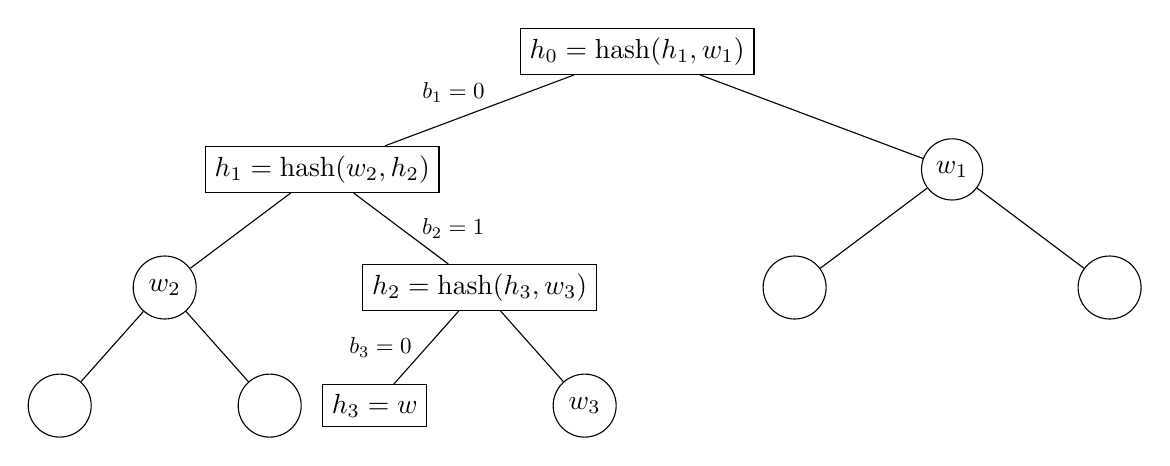
\begin{tikzpicture}[level/.style={sibling distance=8cm/#1}]
\renewcommand{\hash}[1]{\mathrm{hash}({#1})}
\node [rectangle, draw] (c)  {$h_0 = \hash{h_1, w_1}$}
	child { node [rectangle, draw] (l)  {$h_1 = \hash{w_2, h_2}$}  
		child { node [circle, draw, minimum size=0.8cm] (ll) {$w_2$} 
			child { node [circle, draw, minimum size=0.8cm] (lll) {}}
			child { node [circle, draw, minimum size=0.8cm] (llr) {}}
		}
		child { node [rectangle, draw] (B)  {$h_2 = \hash{h_3, w_3}$} 
			child { node [rectangle, draw] (lrl) {$h_3 = w$} 
				edge from parent node[scale=0.83, left=0.1cm] {$b_3= 0$}	
			}
			child { node [circle, draw, minimum size=0.8cm](lrr) {$w_3$}}
			edge from parent node[scale=0.83, right=0.2cm] {$b_2= 1$}	
		}
		edge from parent node[scale=0.83, left=0.4cm, above=0.0cm] {$b_1 = 0$}	
	}
	child { node [circle, draw] (r) {$w_1$}
		child { node [circle, draw, minimum size=0.8cm] (rl) {$$}
		 }
		child { node [circle, draw, minimum size=0.8cm] (rr)  {$$}
		} 
	}
;
\end{tikzpicture}
